\documentclass[12pt, a4paper]{article}
\usepackage[top=2cm, bottom=2cm, right=2.5cm, left=2.5cm]{geometry}
\usepackage[utf8]{inputenc}
\usepackage{amsmath, amsfonts, amssymb}
\usepackage{float}
\usepackage{graphicx}
\usepackage{multicol}
\usepackage{xcolor}
\usepackage{xwatermark}
\usepackage{setspace}
% \newwatermark[allpages, angle=45, scale=2.0, color=black!15]{matematicautodidata.com}

\usepackage{xcolor}  % For styling code colors
\usepackage{listings} % For code blocks

% --- MATLAB Code Styling Configuration ---
\definecolor{commentColor}{RGB}{34,139,34}  % ForestGreen for comments
\definecolor{stringColor}{RGB}{160,32,240}   % Purple for strings
\definecolor{keywordColor}{RGB}{0,0,255}     % Blue for keywords
\definecolor{backgroundColor}{RGB}{248,248,248} % Light gray background

\lstset{
    language=Matlab,
    backgroundcolor=\color{backgroundColor},
    basicstyle=\small\ttfamily,          % Use typewriter/monospaced font
    keywordstyle=\color{keywordColor}\bfseries,
    commentstyle=\color{commentColor},
    stringstyle=\color{stringColor},
    numbers=left,                        % Line numbers on the left
    numberstyle=\tiny\color{gray},       % Line number style
    stepnumber=1,                        % Number every line
    numbersep=8pt,                       % Distance between numbers and code
    frame=single,                        % Draws a frame around the code
    rulecolor=\color{black!20},          % Frame border color
    breaklines=true,                     % Automatically wrap long lines
    breakatwhitespace=false,             % Wrap lines anywhere
    showstringspaces=false,              % Don't show spaces in strings as visual symbols
    keepspaces=true                      % Keeps indentation clean
}

\title{Homework}
\begin{document}
\begin{minipage}[c][2cm][c]{2cm}
	
\includegraphics[height=2cm]{logo.pdf}
\end{minipage}
\begin{minipage}[c][3cm][c]{10cm}
	\center
	{\scriptsize \textit{Sharif University of Technology}}

	% {\scriptsize \textit{Department of Mechanical Engineering}}

	\textbf{\normalsize Medical Robotics}

	{\small{Assignment \#3}}
	\smallskip


\end{minipage}
\begin{minipage}[c][3cm][c]{5cm}
	\footnotesize
	Date: \today

	Dr. Behzadipour


\end{minipage}
\vspace{.5cm}

Mohammad Montazeri \hrulefill \, 404205907

\section*{Part One}
This part the transformation matrix from the image frame to the room frame is calculated analytically with two approaches.
\subsection*{Approach One}
The sequence of transformations that lead to the image frame (I) can be assumed as:
\begin{itemize}
	\item Translations from \(O_0\) to \(O_t\) with \(\vec{O_0 O_t} = [0.2, 4.1, -0.1]^T \,\mathrm{m}\)
	\item Rotation corresponding to Euler XYX angles with \(25^\circ, 15^\circ, 3^\circ\) angles respectively
	\item Translation along X-axis for \(-0.6\,\mathrm{m}\) \footnote{
		      This step points out to the transformation of $t \leftarrow I$ denoted as ($H_I^t$). Frame $I$ is shifted by $-0.6$ along the $x$-axis relative to Frame $t$ ($H_I^t = T_{x}(-0.6)$).Therefore, to go the opposite way—from Frame $I$ back to Frame $t$ ($H_t^I$), one must move in the positive $x$ direction by $0.6$ meters: $H_t^I = (H_I^t)^{-1} = T_{x}(+0.6)$.
	      }
\end{itemize}
Therefore, the overall transformation matrix that maps any point in image coordinates to room coordinates is:
\begin{align}
	H_I^0 & = T_{x, y, z} \, R_{x, y, x} \, T_{x}
\end{align}
where
\begin{align}
	R_{x, y, x}(\alpha, \beta, \gamma) & =         \begin{bmatrix}
		                                               R_{x, 25^\circ}                       & \begin{matrix} 0 \\ 0 \\ 0 \end{matrix} \\
		                                               \begin{matrix} 0 & 0 & 0 \end{matrix} & 1
	                                               \end{bmatrix}
	\begin{bmatrix}
		R_{y, 15^\circ}                       & \begin{matrix} 0 \\ 0 \\ 0 \end{matrix} \\
		\begin{matrix} 0 & 0 & 0 \end{matrix} & 1
	\end{bmatrix}
	\begin{bmatrix}
		R_{x, 3^\circ}                        & \begin{matrix} 0 \\ 0 \\ 0 \end{matrix} \\
		\begin{matrix} 0 & 0 & 0 \end{matrix} & 1
	\end{bmatrix}             \nonumber                                                                                 \\
	                                   & = \begin{bmatrix}
		                                       c\beta          & s\beta s\gamma                            & s\beta c\gamma                            & 0 \\
		                                       s\alpha s\beta  & -s\alpha c\beta s\gamma + c\alpha c\gamma & -s\alpha c\beta c\gamma - c\alpha s\gamma & 0 \\
		                                       -c\alpha s\beta & c\alpha c\beta s\gamma + s\alpha c\gamma  & c\alpha c\beta c\gamma - s\alpha s\gamma  & 0 \\
		                                       0               & 0                                         & 0                                         & 1\end{bmatrix}
\end{align}
Here, with \(\alpha = 25^\circ\), \(\beta = 15^\circ\), and \(\gamma = 3^\circ\), the rotation matrix can be calculated as
\begin{align}
	R_{x, y, x}(25^\circ, 15^\circ, 3^\circ) & = \begin{bmatrix}
		                                             0.9659  & 0.0135 & 0.2584  & 0 \\
		                                             0.1093  & 0.8837 & -0.4550 & 0 \\
		                                             -0.2345 & 0.4678 & 0.8521  & 0 \\
		                                             0       & 0      & 0       & 1
	                                             \end{bmatrix}
\end{align}
So,
\begin{align}
	H_I^0 & =
	\begin{bmatrix}
		I_{3\times3}                          & \begin{matrix} 0.2 \\ 4.1 \\ -0.1 \end{matrix} \\
		\begin{matrix} 0 & 0 & 0 \end{matrix} & 1
	\end{bmatrix}
	\, [R_{x, y, x}]_{4\times4} \,
	\begin{bmatrix}
		I_{3\times3}                          & \begin{matrix} -0.6 \\ 0 \\ 0 \end{matrix} \\
		\begin{matrix} 0 & 0 & 0 \end{matrix} & 1
	\end{bmatrix} \nonumber \\
	      & = \begin{bmatrix}
				0.9659 & 0.0135 & 0.2585 & -0.3796 \\
				0.1094 & 0.8837 & -0.4551 & 4.0344 \\
				-0.2346 & 0.4679 & 0.8521 & 0.0407 \\
				0 & 0 & 0 & 1.0000
	          \end{bmatrix}
\end{align}
To transform any point between the two specified frames, we have
\begin{align}
	P_I^I & = H_0^I P_0^0 \label{eq:1}
\end{align}
According to equation~\ref{eq:1}, \(H_0^I\) gives the transformation from the image frame to the room frame, which is the objective of this problem. To find \(H_0^I\), we can take the inverse of \(H_I^0\). For a homogeneous transformation

\begin{align}
	T=
	\begin{bmatrix}
		R & p \\
		0 & 1
	\end{bmatrix} \label{eq:2}
\end{align}
the inverse is
\begin{align}
	T^{-1}=
	\begin{bmatrix}
		R^T & -R^T p \\
		0   & 1
	\end{bmatrix} \label{eq:3}
\end{align}
So, using the above formula, the inverse of \(H_I^0\) can be calculated as
\begin{align}
	H_0^I & = (H_I^0)^{-1} = \begin{bmatrix}
								0.9659 & 0.1094 & -0.2346 & -0.0651 \\
								0.0135 & 0.8837 & 0.4679 & -3.5791 \\
								0.2585 & -0.4551 & 0.8521 & 1.8994 \\
								0 & 0 & 0 & 1.0000
	                         \end{bmatrix}
\end{align}
\subsection*{Approach Two}
We need to find the homogeneous transformation matrix $H_0^I$ that maps a point from the operating room frame (Frame 0) to the image/graphics software frame (Frame I) [equation~\ref{eq:1}]. We can find the transformation by going from Frame 0 to Frame $t$ (the physical target), and then from Frame $t$ to Frame $I$:
\begin{align}
	H_0^I = H_t^I H_0^t = H_t^I (H_t^0)^{-1} \label{eq:5}
\end{align}
We are given the translation vector and $XYX$ Euler angles for Frame $t$ relative to Frame 0; Thus, the full homogeneous matrix $H_t^0$ and its inverse using equations~\ref{eq:2} and~\ref{eq:3} is:
\begin{align}
	H_t^0        & = \begin{bmatrix} 0.9659 & 0.0135 & 0.2584 & 0.2 \\ 0.1094 & 0.8837 & -0.4550 & 4.1 \\ -0.2346 & 0.4678 & 0.8521 & -0.1 \\ 0 & 0 & 0 & 1 \end{bmatrix}           \\
	(H_t^0)^{-1} & = \begin{bmatrix} 0.9659 & 0.1094 & -0.2346 & -0.6652 \\ 0.0135 & 0.8837 & 0.4678 & -3.5791 \\ 0.2584 & -0.4550 & 0.8521 & 1.8990 \\ 0 & 0 & 0 & 1 \end{bmatrix}
\end{align}

The corresponding coordinate axes in both Frame $t$ and Frame $I$ are parallel, so there is no rotation ($R_t^I = I_{3\times3}$). The origin shifts from one end of the x-axis edge in Frame $t$ to the opposite end in Frame $I$, so the translation is purely along the x-axis by -0.6 meters:
\begin{align}
	H_t^I = \begin{bmatrix} 1 & 0 & 0 & 0.6 \\ 0 & 1 & 0 & 0 \\ 0 & 0 & 1 & 0 \\ 0 & 0 & 0 & 1 \end{bmatrix}
\end{align}
Finally, by forming equation~\ref{eq:5}, the same result as in Approach One can be seen.


\section*{Part Two}
One needs three points to fully determine the position and orientation of the cube. The coordinates of the selected points in the image frame are (figure~\ref{fig:points}):
\begin{align*}
	P_1^I & = [0.6, 0, 0.2]^T \,\mathrm{m} \\
	P_2^I & = [0, 0.3, 0.2]^T \,\mathrm{m} \\
	P_3^I & = [0.6, 0.3, 0]^T \,\mathrm{m}
\end{align*}
\begin{figure}[htbp]
	\centering
	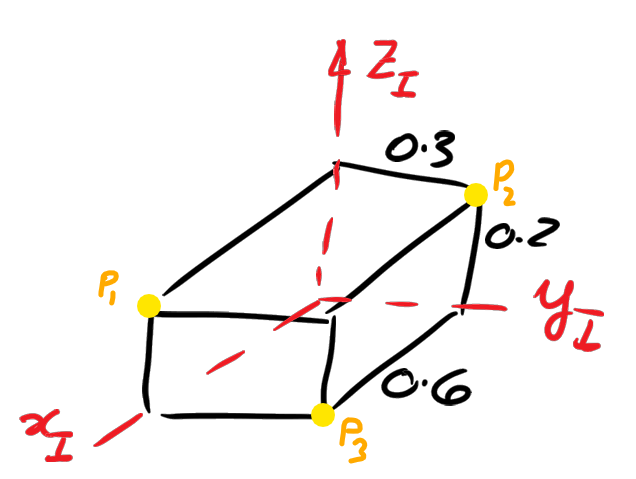
\includegraphics[width=.5\textwidth]{Figure1.png}
	\caption{Selected points in the image frame.}
	\label{fig:points}
\end{figure}

However, three individual points do not provide enough spatial information to uniquely solve for all 12 degrees of freedom in a full $4\times4$ homogeneous transformation matrix if one is going to solve the system of equations in equation~\ref{eq:4} without adding the properties of homogenous rotation matrices. Therefore, a forth point is added to the system by assuming that the origin of the cube in the image frame is located at $P_4^I = [0, 0, 0]^T$.
\begin{align}
	P_i^0 & = H_I^0 P_i^I \quad \forall i = 1,2,3,4 \label{eq:4}
\end{align}
We form this equation for the four selected points and solve for \(H_I^0\) in Matlab.
Using the analytical forward mapping matrix $H_I^0$ derived in previous section, one can calculate the position of selected landmarks in Frame 0 ($\vec{P}^0 = H_I^0 \vec{P}^I$).
Afterwards, to solve for the 12 unknown parameters of $H_I^0$ using point correspondences, we isolate each coordinate dimension ($x, y, z$) into decoupled linear systems of the form $A \, X = B$.
\begin{align*}
	A = \begin{bmatrix}
		    (\vec{P}_1^I)^T \\ (\vec{P}_2^I)^T \\ (\vec{P}_3^I)^T \\ (\vec{P}_4^I)^T
	    \end{bmatrix} =
	\begin{bmatrix}
		0.6 & 0   & 0.2 & 1 \\
		0   & 0.3 & 0.2 & 1 \\
		0.6 & 0.3 & 0   & 1 \\
		0   & 0   & 0   & 1
	\end{bmatrix}
\end{align*}
The target output matrix $B$ collects the measured tracking positions in the room:
\begin{align}
	B = \begin{bmatrix} x_{1}^0 & y_{1}^0 & z_{1}^0 \\ x_{2}^0 & y_{2}^0 & z_{2}^0 \\ x_{3}^0 & y_{3}^0 & z_{3}^0 \\ x_{4}^0 & y_{4}^0 & z_{4}^0 \end{bmatrix} =
	\begin{bmatrix}
		0.4675 & -3.4774 & 2.2249 \\
		-0.0792 & -3.2204 & 1.9333 \\
		0.5473 & -3.3059 & 1.9179 \\
		-0.0651 & -3.5791 & 1.8994
	\end{bmatrix}
\end{align}
The answer to the system of equations $A_{4\times4} \, X_{4\times3} = B_{4\times3}$ is calculated in Matlab with

\begin{lstlisting}
H_parameters = (A \ B)';
H_I_0 = [H_parameters; 
         0, 0, 0, 1];
\end{lstlisting}

The code is appended to this report and shows the same result for part two and both approaches of part one.

% \begin{thebibliography}{99}
% \bibitem{Michelin2002}
% M.~Michelin, E.~Dombre, P.~Poignet, F.~Pierrot, and L.~Eckert,
% ``Path Planning under a Penetration Point Constraint for Minimally Invasive Surgery,''
% in \textit{Proceedings of the IEEE/RSJ International Conference on Intelligent Robots and Systems (IROS)}, Lausanne, Switzerland, 2002, pp.~1475--1480.
% \end{thebibliography}


\end{document}